% !TEX TS–program = pdflatexmk
\documentclass[12pt,a4paper,oneside,openany]{article}
\usepackage[squaren]{SIunits}
%% LaTeX Preamble - Common packages
\usepackage[english]{babel}
\usepackage{setspace}

\usepackage{fancyhdr}
\pagestyle{fancy}
%\cfoot{\thepage{} – CONFIDENTIAL}


\usepackage[utf8]{inputenc} % Any characters can be typed directly from the keyboard, eg éçñ
\usepackage{textcomp} % provide lots of new symbols
\usepackage{graphicx}  % Add graphics capabilities
\usepackage{flafter}  % Don't place floats before their definition
%\usepackage{topcapt}   % Define \topcaption for placing captions above tables (not in gwTeX)
%\usepackage{natbib} % use author/date bibliographic citations
%\usepackage{babelbib}
\usepackage[backend=biber]{biblatex}
\addbibresource{nanoscan-vs-smps.bib}

\usepackage{subfig}
\usepackage{caption}
\usepackage{enumitem}

\usepackage{amsmath,amssymb}  % Better maths support & more symbols
\usepackage{bm}  % Define \bm{} to use bold math fonts
\usepackage{esint}
\usepackage{algorithm}
\usepackage{mathenv}
%\usepackage[noend]{algorithmic}
\usepackage{algorithmicx}
\usepackage{algpseudocode}
\usepackage[usenames,dvipsnames]{color} 

\usepackage[pdftex,bookmarks,colorlinks,breaklinks]{hyperref}  % PDF hyperlinks, with coloured links
%\definecolor{dullmagenta}{rgb}{0.4,0,0.4}   % #660066
%\definecolor{darkblue}{rgb}{0,0,0.4}
\hypersetup{linkcolor=red,citecolor=blue,filecolor=blue,urlcolor=blue} % coloured links
%\hypersetup{linkcolor=black,citecolor=black,filecolor=black,urlcolor=black} % black links, for print output

\usepackage{memhfixc}  % remove conflict between the memoir class & hyperref
% \usepackage[activate]{pdfcprot}  % Turn on margin kerning (not in gwTeX)
%\usepackage{pdfsync}  % enable tex source and pdf output syncronicity

\usepackage{booktabs}
\usepackage{listings}
\usepackage{nomencl}
\usepackage{todonotes}

\usepackage[noabbrev]{cleveref}

\usepackage{tablefootnote}
%\makesavenoteenv{tabular}

\usepackage{tikz}
\usetikzlibrary{calc,arrows,through,backgrounds,fit,shapes.geometric,shapes.misc,plotmarks,positioning,trees}
\usepackage{circuitikz}

%\usepackage{sagetex}

%\usepackage{anysize}
%\marginsize{2cm}{2cm}{2cm}{2cm}

\onehalfspacing

\makenomenclature
\def\nomlabel#1{\textbf{#1}\hfil}

%\newcommand{\Parameters}{\subsection*{Parameters}}
%\newcommand{\ReturnValue}{\subsection*{Return Value}}
%\newcommand{\Description}{\subsection*{Description}}
%\newcommand{\ClassName}[1]{{\tt #1}}
%\newcommand{\ReturnType}[1]{{\tt (#1)}}
%\newcommand{\Function}[1]{{\tt #1()}}
%\newcommand{\Self}{{\tt self}}

\DeclareMathOperator{\ud}{d}
\DeclareMathOperator{\udt}{\frac{d}{dt}}
%\DeclareMathOperator{\udtt}{\frac{\ud^2}{\ud t^2}}
\DeclareMathOperator{\rank}{rank}
\DeclareMathOperator{\fclamp}{clamp}
\DeclareMathOperator{\fsign}{sign}
%\newcommand{\ud}{\ensuremath{\binop{\mathrm{d}}}}
\newcommand{\vx}{\ensuremath{\boldsymbol{x}}}
\newcommand{\vv}{\ensuremath{\boldsymbol{v}}}
\newcommand{\va}{\ensuremath{\boldsymbol{a}}}
\newcommand{\vf}{\ensuremath{\boldsymbol{f}}}
\newcommand{\vt}{\ensuremath{\boldsymbol{t}}}
\newcommand{\vk}{\ensuremath{\boldsymbol{k}}}
\newcommand{\mM}{\ensuremath{\boldsymbol{M}}}
\newcommand{\mW}{\ensuremath{\boldsymbol{W}}}
\newcommand{\mJ}{\ensuremath{\boldsymbol{J}}}
\newcommand{\mA}{\ensuremath{\boldsymbol{A}}}
\newcommand{\vq}{\ensuremath{\boldsymbol{q}}}
\newcommand{\vC}{\ensuremath{\boldsymbol{C}}}
\newcommand{\vQ}{\ensuremath{\boldsymbol{Q}}}
\newcommand{\vlambda}{\ensuremath{\boldsymbol{\lambda}}}
\newcommand{\vd}{\ensuremath{\boldsymbol{d}}}
\newcommand{\mI}{\ensuremath{\boldsymbol{I}}}
\newcommand{\vc}{\ensuremath{\boldsymbol{c}}}
\newcommand{\vr}{\ensuremath{\boldsymbol{r}}}
\newcommand{\vF}{\ensuremath{\boldsymbol{F}}}
\newcommand{\vtau}{\ensuremath{\boldsymbol{\tau}}}
\newcommand{\valpha}{\ensuremath{\boldsymbol{\alpha}}}

\newtheorem{mydef}{Definition}


\lstset{numbers=left,basicstyle=\footnotesize\ttfamily,numberstyle=\tiny,tabsize=4,breaklines=true}
\lstset{language=[Objective]C}
\lstset{commentstyle=\color{BrickRed}\itshape,
	keywordstyle=\color{RoyalBlue}\bfseries,
	identifierstyle=\color{Blue},
	stringstyle=\color{Gray}}

\long\def\symbolfootnote[#1]#2{\begingroup%
\def\thefootnote{\fnsymbol{footnote}}\footnote[#1]{#2}\endgroup}


\begin{document}


\title{Servo Controller Design Notes}
\author{Dömötör Gulyás\\v0.1}

\maketitle

%\abstract
%
%foopsum.
%
%

\tableofcontents

%\listoffigures

%\section{Introduction}

%\begin{figure}[htbp]
%\begin{center}
%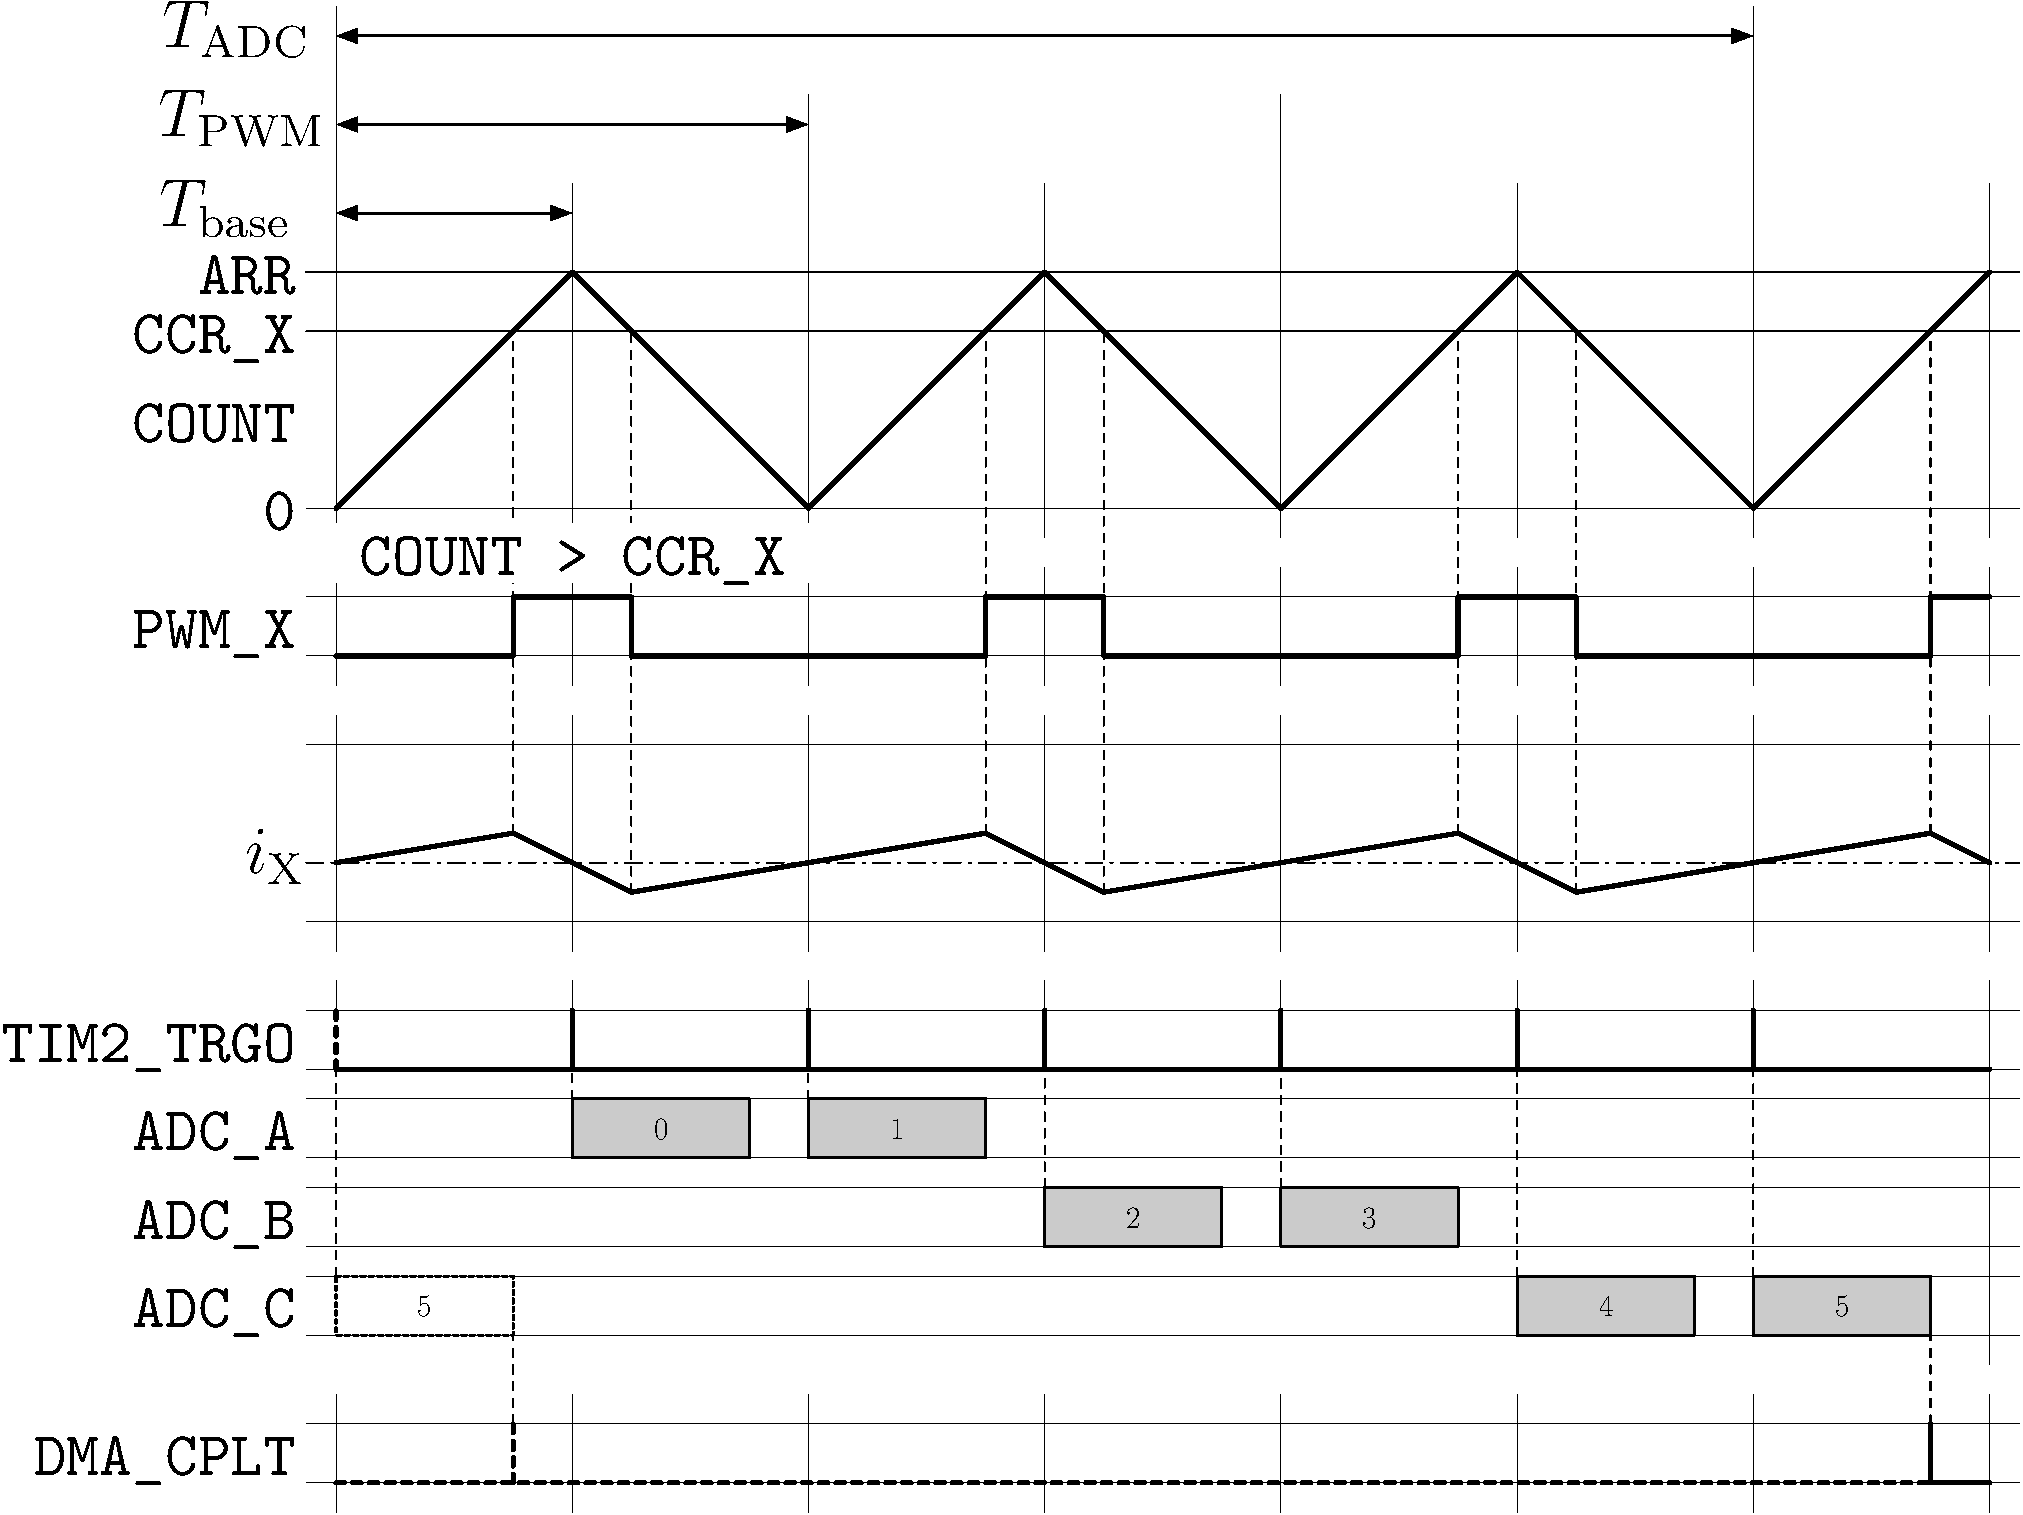
\includegraphics[scale=0.8]{n17-servo-pwm-adc.pdf}
%\caption[Fig]{foo}
%\label{fig:pwm-adc}
%\end{center}
%\end{figure}

\section{Hardware}

The hardware is laid out to be as flexible as possible, driving both 3-phase BLDC and servo motors, as well as 2-phase steppers.

3 half bridges with discrete transistors allow high currents. The DRV8323 stepper driver works at up to 60V. The hardware is laid out for 12V-48V nominal voltage, but allowing 60V peak.

Using a 2-phase motor in this configuration limits the top speed due to lower effective voltage than one could get using 2 full bridges.

The main MCU is an STM32G431.

\subsubsection{MCU Peripheral Assignments}

\begin{table}[htbp]
\caption{MCU Peripheral Usage}
\begin{center}
\begin{tabular}{|l|l|}
\hline Peripheral & Usage \\
\hline \texttt{ADC1} & Auxiliary analog inputs \\
\texttt{ADC2} & Current Sensing \\
\hline
\texttt{TIM2} & PWM Gate Driver (R,A,B,C) \\
\texttt{TIM3} & Encoder Input \\
\texttt{TIM4} & RGB LED PWM \\
\texttt{TIM6} & Performance Counter / Timer \\
\texttt{TIM15} & current sense trigger offset \\
\hline
\texttt{I2C3} & I2C I/O \\
\texttt{USART1} & Debug I/O \\ 
\texttt{SPI2} & Gate Driver and Magnetic Encoder \\
\texttt{USB} & USB Interface \\
\hline
\end{tabular}
\end{center}
\label{tab:mcu-peripherals}
\end{table}%


\section{PWM and Current Sensing}

\begin{figure}[htbp]
\begin{center}
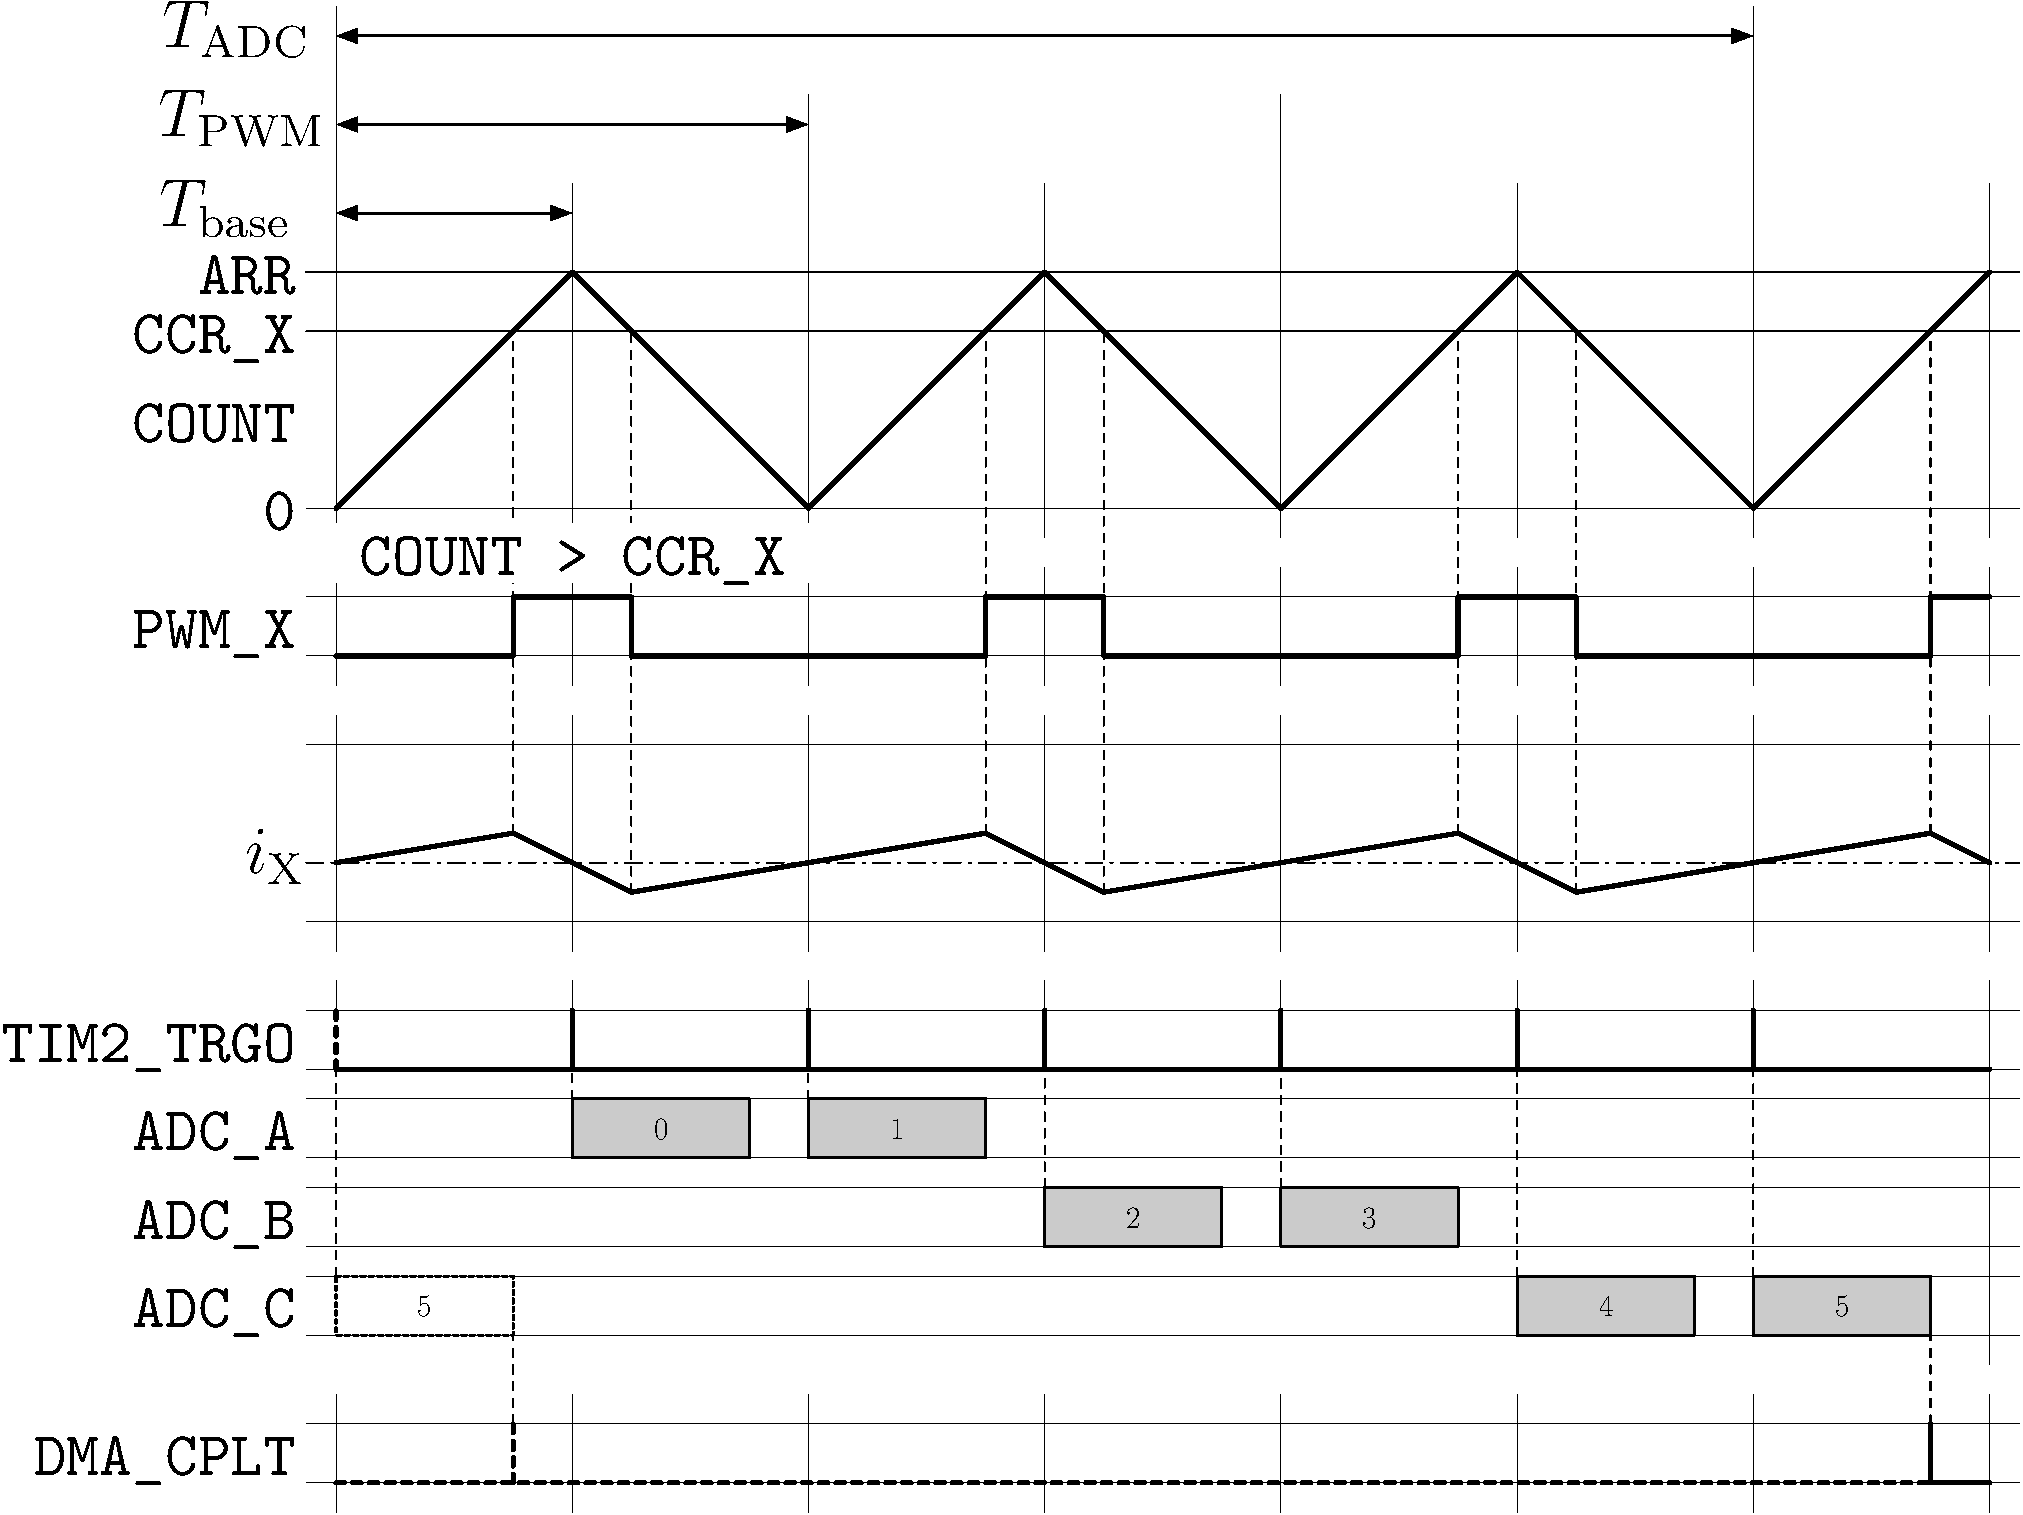
\includegraphics[scale=0.4]{n17-servo-pwm-adc.pdf}
\caption[PWM and ADC Sync]{Temporal synchronization of PWM output and ADC sampling.}
\label{fig:pwm-adc}
\end{center}
\end{figure}

\section{PWM}

The PWM output has to be synchronized with sampling the current sense values. This is done through builtin hardware trigger mechanisms between the different peripherals on the MCU which allow precise timing without CPU involvement.

ADC sampling should happen in the middle of the PWM high/low periods, and to achieve this PWM is run in up/down counting mode, and the ADC readout is triggered at the end of each period.

The PWM base period $T_{\textrm{base}} = \unit{10}{\micro\second}$ ($f_{\textrm{base}} = \unit{100}{\kilo\hertz}$) results in an effective output period of $T_{\textrm{gate}} = \unit{20}{\micro\second}$ ($f_{\textrm{gate}} = \unit{50}{\kilo\hertz}$), and ADC sampling of each channel every $T_{\textrm{sense}} = \unit{60}{\micro\second}$ ($f_{\textrm{sense}} = \unit{16.7}{\kilo\hertz}$).

\texttt{TIM2} is setup for driving the gate driver and brake resistor PWM.

\section {ADC}

\subsubsection{ADC Sampling}

\texttt{ADC2} is setup to sample with 12.5 cycles sample time, with 16x oversampling. $f_{\textrm{ADC}} = \unit{170/3}{\mega\hertz}$, and a single channel takes $12.5+12.5$ cycles per sample\footnote{sampling plus conversion}, with $T_{\textrm{sample}} = \unit{0.44}{\micro\second}$. That ends up being $T_{\textrm{ssaa}} = \unit{7.06}{\micro\second}$ with 16x oversampling.

Positive currents can only be measured in low periods, when the lower switch is closed, but negative currents can be measured in both high and low periods, as the body diode will always conduct.

\subsubsection{ADC Triggering}

As the ADC sampling takes a finite time, it will not quite sample on-center. \texttt{TIM15} is setup to offset by $T_{\textrm{base}} - T_{\textrm{ssaa}}/2 = \unit{6.47}{\micro\second}$ or 1100 CPU cycles.

\begin{figure}[htbp]
\begin{center}
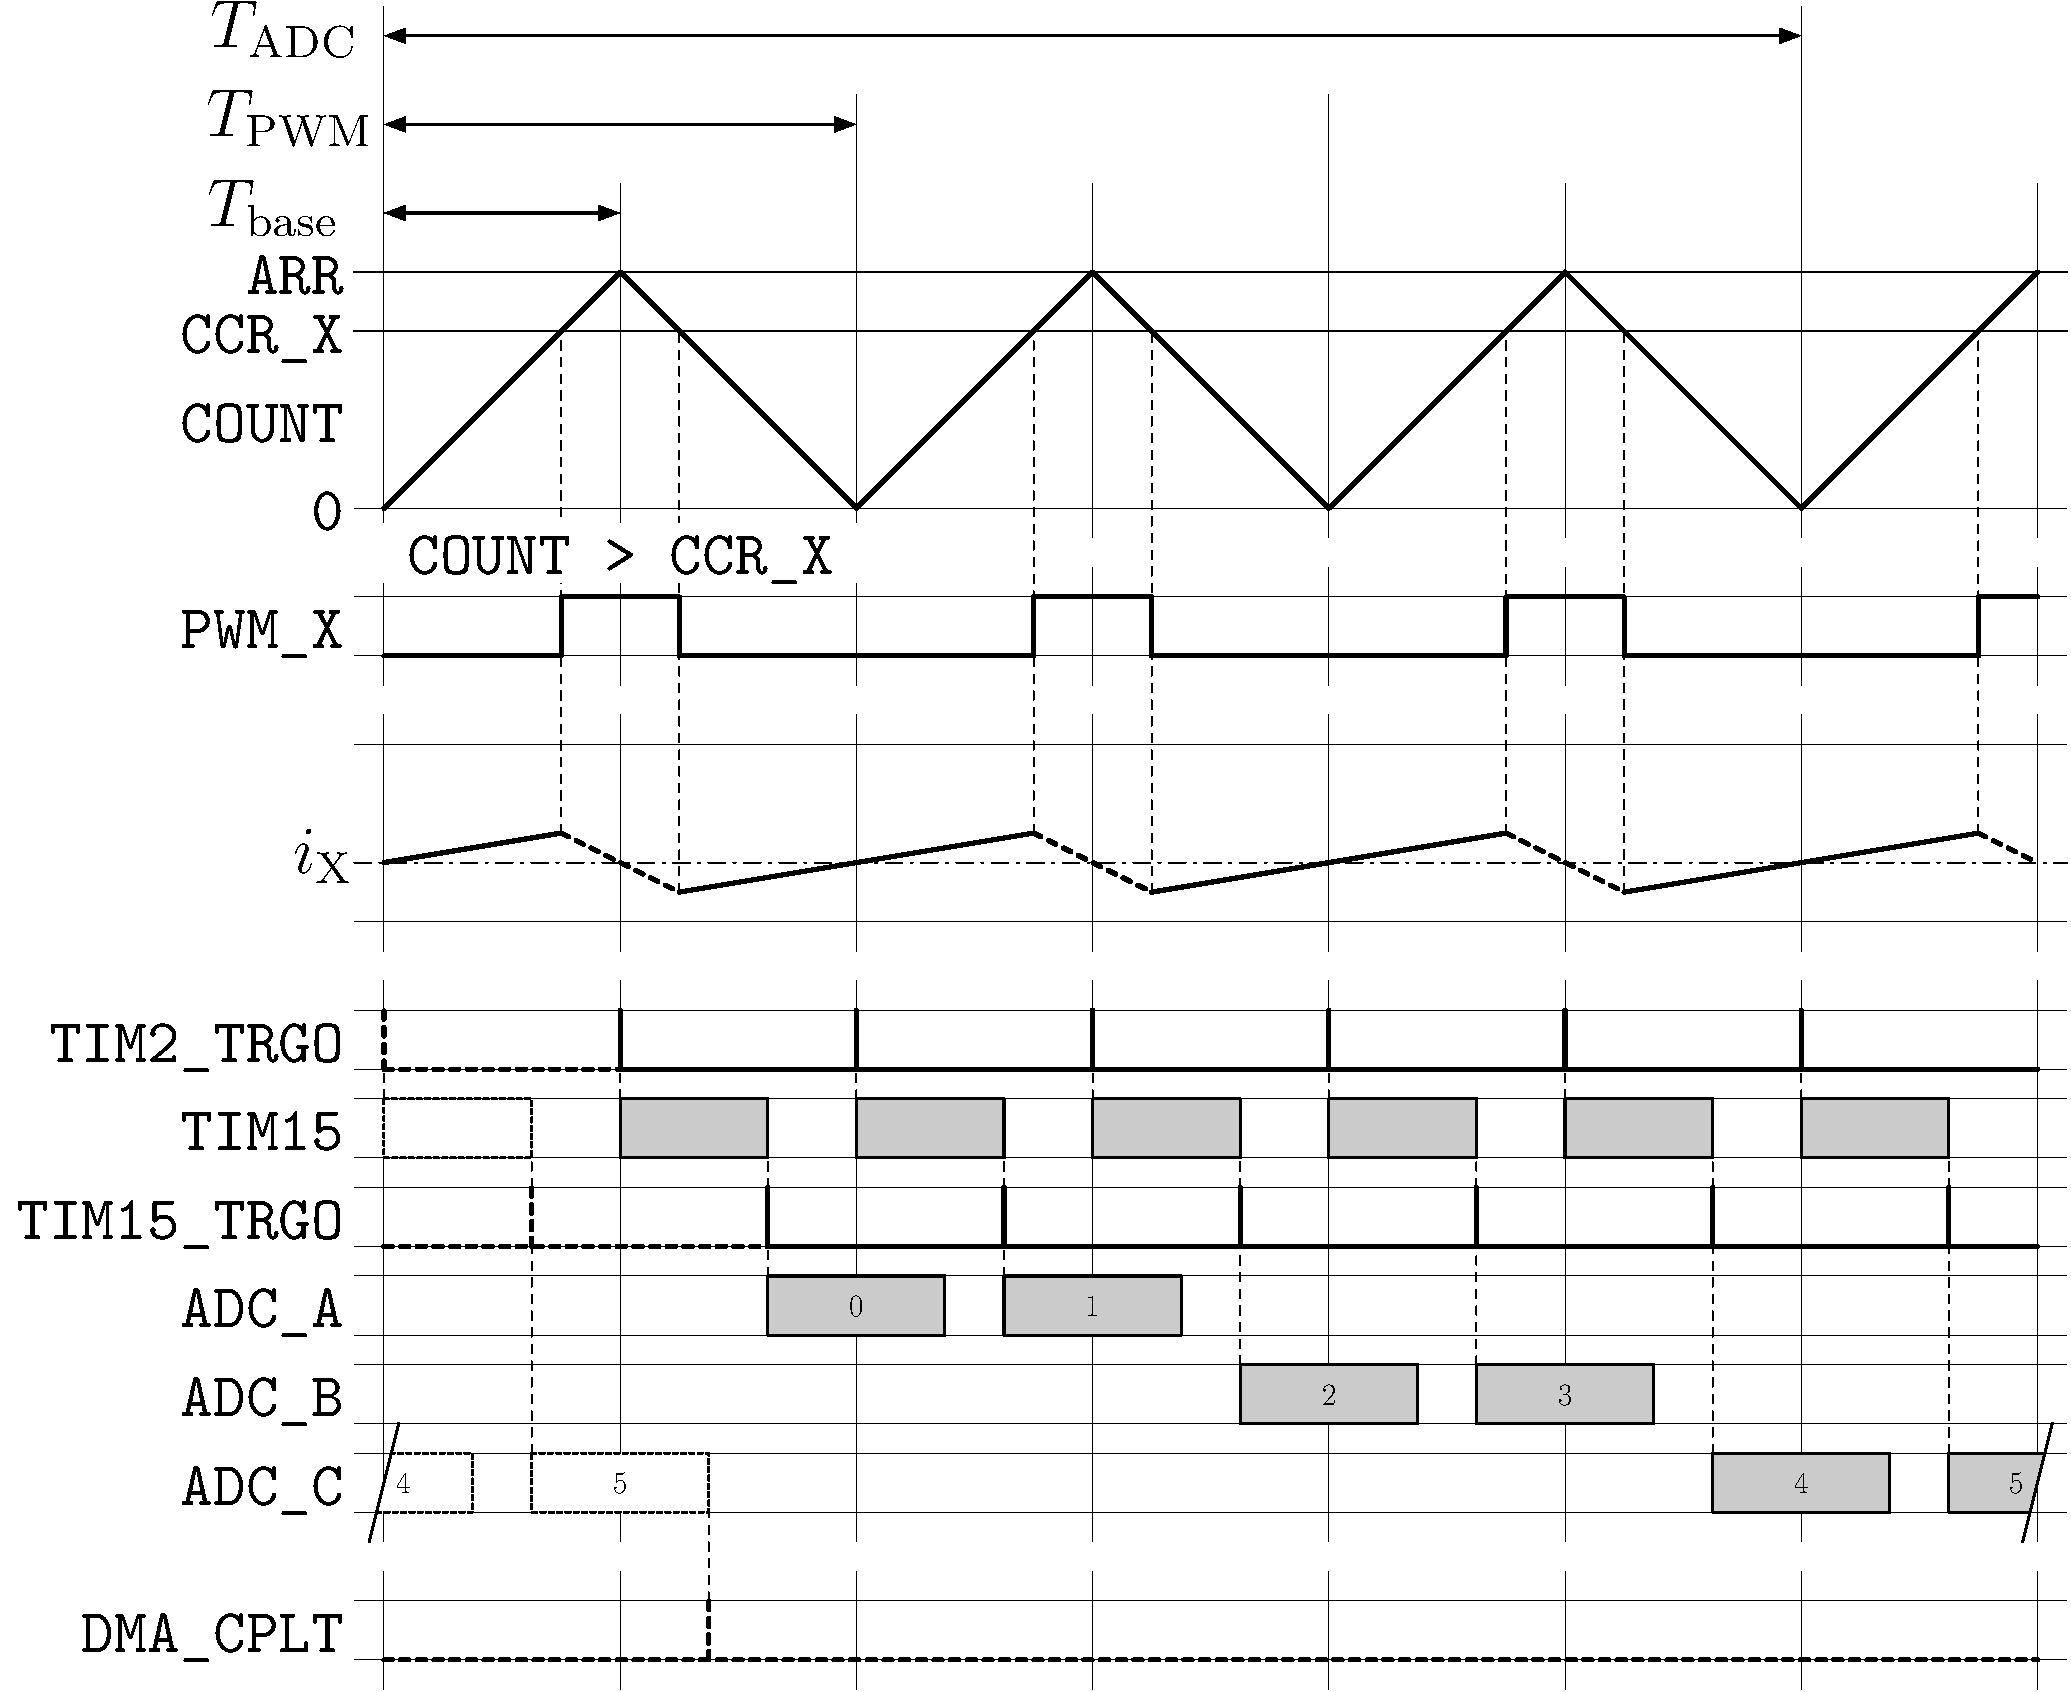
\includegraphics[scale=0.4]{n17-servo-pwm-adc-offset.pdf}
\caption[PWM and ADC Sync with Offset]{Temporal synchronization of PWM output and ADC sampling with centering offset. Adding a triggered timer as a delay allows offsetting the ADC sampling to occur centered on PWM phases.}
\label{fig:pwm-adc-offset}
\end{center}
\end{figure}


\section{The RL-Circuit}

\begin{figure}[htbp]
\begin{center}
\begin{circuitikz} \draw
(0,0) to[european voltage source, v=U] (0,4) -- (4,4)
  to[L,l=L,i=i] (4,2)
  to[R,l=R] (4,0) -- (0,0)
;
\end{circuitikz}
\caption[RL Circuit]{RL Circuit Diagram}
\label{fig:RL}
\end{center}
\end{figure}


The governing equation of an RL Series Circuit is 
\begin{align}
\frac{\ud}{\ud t} i &= \frac{U - R i}{L} \\
\frac{\ud^2}{\ud t^2} i &= -\frac{R}{L} \frac{\ud}{\ud t} i
\end{align}
%which can be combined to form
%\begin{align}
%-\frac{L}{R} \frac{\ud^2}{\ud t^2} i &= \frac{U - R i}{L}
%\end{align}
%and simplified to
%\begin{align}
%-\frac{L^2}{R^2} \frac{\ud^2}{\ud t^2} i &= \frac{U}{R} - i\\
%L^2 \frac{\ud^2}{\ud t^2} i &= iR^2 - UR
%\end{align}

\subsubsection{Time Domain}

\begin{align}
i R&= U \left( 1 - e^{-t\frac{R}{L}} \right)
\end{align}


\begin{align}
i &= \frac{U}{R} \left( 1 - e^{-t\frac{R}{L}} \right) \\
\frac{\ud}{\ud t} \imath &= \frac{U}{L} e^{-t\frac{R}{L}} \\
\frac{\ud^2}{\ud t^2} \imath &= -\frac{UR}{L^2} e^{-t\frac{R}{L}}
\end{align}

Logarithmic linear regression of first/second derivative?
\begin{align}
\log \left(\frac{L}{U} \frac{\ud}{\ud t} \imath \right) &= -t\frac{R}{L} \\
\log \left( L \right) - \log \left(U \right) + \log \left(\frac{\ud}{\ud t} \imath \right) &= -t\frac{R}{L} \\
\frac{\ud^2}{\ud t^2} \imath &= -\frac{UR}{L^2} e^{-t\frac{R}{L}}
\end{align}



\subsubsection{Combining for L}

Rearranging both equations to be able to drop $R$
\begin{align}
\frac{R}{L} &= \frac{\frac{U}{L} - \dot{\imath}}{\imath} \\
\frac{R}{L} &= - \frac{ \ddot{\imath}}{ \dot{\imath}}
\end{align}
and combining
\begin{align}
\frac{\frac{U}{L} -  \dot{\imath}}{\imath} &= - \frac{\ddot{\imath}}{ \dot{\imath}} \\
\frac{U}{L} -  \dot{\imath} &= - \frac{\ddot{\imath}}{\dot{\imath}} \imath \\
\frac{U}{L}  \dot{\imath} - \dot{\imath}^2 &= - \ddot{\imath} \imath \\
\frac{U}{L}  \dot{\imath} &= \dot{\imath}^2 - \ddot{\imath} \imath \\
L &= U \frac{ \dot{\imath}}{ \dot{\imath}^2 - \ddot{\imath} \imath}
\end{align}

\subsubsection{Combining for R}
\begin{align}
- R \frac{\dot{\imath}}{\ddot{\imath}} &= U \frac{ \dot{\imath}}{ \dot{\imath}^2 - \ddot{\imath} \imath} \\
- R &= U \frac{ \ddot{\imath}}{ \dot{\imath}^2 - \ddot{\imath} \imath}
\end{align}

\subsubsection{Time Constant}

The above formulas for $R$ and $L$ show that the only difference is the appearance of the first vs. second differential of the current in the nominator. As the current curve is an exponential function, both differentials have the same shape, but differ in magnitude by $\tau=R/L$, and thus 
\begin{align}
\tau &= - \frac{\ddot{\imath}}{\dot{\imath}}
\end{align}

\subsection{LR Estimation}

Sampling a  applied voltage $U$ step function at fixed intervals $T$, for samples $i_0, i_1, \ldots, i_n$ with t $t>0,n=t/T$, we can compute the differentiations in different ways.

\subsubsection{N3 Sampling}

Assuming linearity around $n=1$:
\begin{align}
{\imath} &= \frac{1}{3} (\imath_0 + \imath_1 + \imath_2) \\
\dot{\imath} &= \frac{1}{2T} (\imath_2 - \imath_0) \\
\ddot{\imath} &= \frac{1}{T^2} (\imath_2 - 2\imath_1 + \imath_0)
\end{align}
and
\begin{align}
L &= U \frac{\dot{\imath}}{\dot{\imath}^2 - \ddot{\imath} \imath}
\end{align}



\section{2-Phase Motor With 3-Phase Driver}

In theory, all motor parameters can be estimated by sequentially turning one half bridge low, while the others are switched high, allowing current to simultaneously flow in in two places, but only out in one. However, the parameter estimation is difficult with noisy values.

\subsection{Full Dynamic Circuit}

\begin{figure}[htbp]
\begin{center}
\begin{circuitikz} 
\draw (0,8) 
  to[R,] ++(0,-2)
  to[normal open switch,] ++(0,-1)
  to[R,] ++(0,-2)
  to[R,] ++(0,-2)
  to[normal open switch,l=$A$] ++(0,-1)
;
\draw (4,8) node[vcc]{U}
  to[R,] ++(0,-2)
  to[normal open switch,] ++(0,-1)
  to[R,] ++(0,-2)
  to[R,] ++(0,-2)
  to[normal open switch,l=$B$] ++(0,-1)
  node[rground]{}
;
\draw (8,8) 
  to[R,l=$R_T$] ++(0,-2)
  to[normal open switch,] ++(0,-1)
  to[R,l=$R_T$] ++(0,-2)
  to[R,l=$R_S$] ++(0,-2)
  to[normal open switch,l=$C$] ++(0,-1)
;
\draw (0,0)
  to[short,-*] ++(4,0)
  to[short] ++(4,0)
;
\draw (0,5)
  to[R,l=$R_P$,*-] ++(2,0)
  to[L,l=$L_P$,] ++(2,0)
  to[R,*-] ++(2,0)
  to[L,-*] ++(2,0)
;
\draw (0,8)
  to[short,-*] ++(4,0)
  to[short] ++(4,0)
;

\end{circuitikz}
\caption[ABBC Driver]{3-Phase Driver with 2-Phase Motor with phase resistance $R_P$ and switching resistance $R_T$ and shunt resistance $R_S$.}
\label{fig:ABBC}
\end{center}
\end{figure}




\begin{figure}[htbp]
\begin{center}
\begin{circuitikz} 
\draw (0,8) 
  to[R,] ++(0,-2)
  to[normal open switch,] ++(0,-1)
  to[R] ++(0,-2)
  to[R,f=$i_A$] ++(0,-2)
  to[short,l=$A$] ++(0,-1)
;
\draw (4,8) node[vcc]{U}
  to[R,f=$i_b$] ++(0,-2)
  to[short,] ++(0,-1)
  to[R,] ++(0,-2)
  to[R,] ++(0,-2)
  to[normal open switch,l=$B$] ++(0,-1)
  node[rground]{}
;
\draw (8,8) 
  to[R,l=$R_T$,f=$i_c$] ++(0,-2)
  to[short,] ++(0,-1)
  to[R,l=$R_T$,] ++(0,-2)
  to[R,l=$R_S$,] ++(0,-2)
  to[normal open switch,l=$C$] ++(0,-1)
;
\draw (0,0)
  to[short,-*] ++(4,0)
  to[short] ++(4,0)
;
\draw (0,5) node[circ,label={[shift={(-0.4,0.0)}]:{$U_a$}}]{}
  to[R,l_=$R_P$,*-] ++(2,0)
  to[L,l_=$L_P$,] ++(2,0) node[circ,label={[shift={(-0.3,0.0)}]:{$U_b$}}]{}
  to[R,-] ++(2,0)
  to[L,-*] ++(2,0) node[circ,label={[shift={(-0.3,0.0)}]:{$U_c$}}]{}
;
\draw (0,8)
  to[short,-*] ++(4,0)
  to[short] ++(4,0)
;

\end{circuitikz}
\caption[ABBC Driver]{Half-Bridge $A$ switched on low, with $B,C$ switched on high creating asymmetric currents across both phases.
}
\label{fig:ABBC-A}
\end{center}
\end{figure}

For the 2-Phase circuit switched as in \cref{fig:ABBC-A} the governing equations with unknowns $i_b,i_c,U_b$ are
\begin{align}
U_b &= L_P \udt i_A + i_A (R_T + R_S + R_P) \\
U-U_b &= i_b R_T \\
U-U_b &= L_P \udt i_c + i_c (R_T + R_P) \\
i_A &= i_b + i_c
\end{align}
and rearranging 
\begin{align}
\udt i_A  &= \frac{U - i_b R_T - i_A (R_T + R_S + R_P)}{L_P} \\
\udt (i_A - i_b)  &= \frac{i_b R_T - (i_A - i_b) (R_T + R_P)}{L_P}
\end{align}
and Laplace transforming
\begin{align}
s I_A(s)  &= \frac{U - I_b(s) R_T - I_A(s) (R_T + R_S + R_P)}{L_P} \\
s \left( I_A(s) - I_b(s) \right) &= \frac{I_b(s) R_T - \left(I_A(s) - I_b(s)\right) (R_T + R_P)}{L_P}
\end{align}
and rearranging
\begin{align}
L_P s I_A(s)  &= U - I_b(s) R_T - I_A(s) (R_T + R_S + R_P) \\
L_P s \left( I_A(s) - I_b(s) \right) &= 2 I_b(s) R_T + I_b(s) R_p - I_A(s) (R_T + R_P)
\end{align}
and again
\begin{align}
R_T I_b(s) &= U - (L_P s + R_T + R_S + R_P) I_A(s)  \\
\left(L_P s + 2 R_T + R_P\right) I_b(s) &= (L_P s + R_T + R_P) I_A(s) 
\end{align}
and combining
\begin{align}
\frac{(L_P s + R_T + R_P)}{L_P s + 2 R_T + R_P} I_A(s)&= \frac{U - (L_P s + R_T + R_S + R_P) I_A(s)}{R_T}
\end{align}
and rearranging
\begin{align}
\left( \frac{(L_P s + R_T + R_P)}{L_P s + 2 R_T + R_P} + \frac{L_P s + R_T + R_S + R_P}{R_T} \right) I_A(s) &= \frac{U}{R_T}
\end{align}
and rearranging
\begin{align}
\left( R_T (L_P s + R_T + R_P) \right. \\
+ &\left (L_P s + R_T + R_S + R_P) (L_P s + 2 R_T + R_P) \right) I_A(s) \\
 = &(L_P s + 2 R_T + R_P) U
\end{align}
expanding
\begin{gather}
\begin{aligned}
\left( R_T L_P s + R_T^2 + R_P R_T \right. \\
+ & L_P^2 s^2 + R_T L_P s + R_S L_P s + R_P L_P s \\
+ & R_T L_P s + 2R_T^2 + R_P R_T \\
+ & R_S L_P s + 2 R_S R_T + R_P R_S\\
+ &\left. R_P L_P s + 2 R_P R_T + R_P^2 \right) I_A(s) \\
 = (L_P s + 2 R_T + R_P) U
\end{aligned}
\end{gather}
simplifying
\begin{gather}
\begin{aligned}
\left( L_P^2 s^2 + 2 R_S L_P s + 2 R_P L_P s + 3 R_T L_P s \right. \\
+ \left. 2 R_S R_T + R_P R_S + R_P^2 + 3 R_T^2 + 4 R_P R_T\right) I_A(s) \\
 = & (L_P s + 2 R_T + R_P) U
\end{aligned}
\end{gather}

\subsection{Resistive Static Circuit}

\begin{figure}[htbp]
\begin{center}
\begin{circuitikz} 
\draw (0,8) 
  to[R,] ++(0,-2)
  to[normal open switch,] ++(0,-1)
  to[R,] ++(0,-2)
  to[R,] ++(0,-2)
  to[normal open switch,l=$A$] ++(0,-1)
;
\draw (4,8) node[vcc]{U}
  to[R,] ++(0,-2)
  to[normal open switch,] ++(0,-1)
  to[R,] ++(0,-2)
  to[R,] ++(0,-2)
  to[normal open switch,l=$B$] ++(0,-1)
  node[rground]{}
;
\draw (8,8) 
  to[R,l=$R_T$] ++(0,-2)
  to[normal open switch,] ++(0,-1)
  to[R,l=$R_T$] ++(0,-2)
  to[R,l=$R_S$] ++(0,-2)
  to[normal open switch,l=$C$] ++(0,-1)
;
\draw (0,0)
  to[short,-*] ++(4,0)
  to[short] ++(4,0)
;
\draw (0,5)
  to[R,l=$R_P$,*-] ++(4,0)
  to[R,*-*] ++(4,0)
;
\draw (0,8)
  to[short,-*] ++(4,0)
  to[short] ++(4,0)
;

\end{circuitikz}
\caption[ABBC Driver Static]{3-Phase Driver with 2-Phase Motor static resistive circuit.}
\label{fig:ABBC-R}
\end{center}
\end{figure}

\begin{figure}[htbp]
\begin{center}
\subfloat[A switched low.]{
\begin{circuitikz} 
\draw (0,8) 
  to[R,] ++(0,-2)
  to[normal open switch,] ++(0,-1)
  to[R] ++(0,-2)
  to[R,f=$i_A$] ++(0,-2)
  to[short,l=$A$] ++(0,-1)
;
\draw (2,8) node[vcc]{U}
  to[R,f=$i_b$] ++(0,-2)
  to[short,] ++(0,-1)
  to[R,] ++(0,-2)
  to[R,] ++(0,-2)
  to[normal open switch,l=$B$] ++(0,-1)
  node[rground]{}
;
\draw (4,8) 
  to[R,l=$R_T$,f=$i_c$] ++(0,-2)
  to[short,] ++(0,-1)
  to[R,l=$R_T$,] ++(0,-2)
  to[R,l=$R_S$,] ++(0,-2)
  to[normal open switch,l=$C$] ++(0,-1)
;
\draw (0,0)
  to[short,-*] ++(2,0)
  to[short] ++(2,0)
;
\draw (0,5)
  to[R,l_=$R_P$,*-*] ++(2,0)
  to[R,-] ++(2,0) 
;
\draw (0,8)
  to[short,-*] ++(2,0)
  to[short] ++(2,0)
;

\end{circuitikz}
}%
~
\subfloat[B switched low.]{
\begin{circuitikz} 
\draw (0,8) 
  to[R,f=$i_a$] ++(0,-2)
  to[short,] ++(0,-1)
  to[R] ++(0,-2)
  to[R,] ++(0,-2)
  to[normal open switch,l=$A$] ++(0,-1)
;
\draw (2,8) node[vcc]{U}
  to[R,] ++(0,-2)
  to[normal open switch,] ++(0,-1)
  to[R,] ++(0,-2)
  to[R,f=$i_B$] ++(0,-2)
  to[short,l=$B$] ++(0,-1)
  node[rground]{}
;
\draw (4,8) 
  to[R,l=$R_T$,f=$i_c$] ++(0,-2)
  to[short,] ++(0,-1)
  to[R,l=$R_T$,] ++(0,-2)
  to[R,l=$R_S$,] ++(0,-2)
  to[normal open switch,l=$C$] ++(0,-1)
;
\draw (0,0)
  to[short,-*] ++(2,0)
  to[short] ++(2,0)
;
\draw (0,5)
  to[R,l_=$R_P$,*-*] ++(2,0)
  to[R,-] ++(2,0) 
;
\draw (0,8)
  to[short,-*] ++(2,0)
  to[short] ++(2,0)
;

\end{circuitikz}
}
\caption[ABBC-RAB]{Resistive Half-Bridge switched low on $A,B$ phases, respectively.
}
\label{fig:ABBC-RAB}
\end{center}
\end{figure}

For the 2-Phase circuit switched as in \cref{fig:ABBC-RAB} the measureable resistances are
\begin{gather}
\begin{aligned}
R_A &= R_S + R_T + R_P + \frac{R_T (R_T + R_P)}{2 R_T + R_P} \\
R_B &= R_S + R_T + \frac{R_T + R_P}{2}
\end{aligned}
\end{gather}
which allows us to solve for $R_T, R_P$ with $R_S$ being known:
\begin{gather}
\begin{aligned}
(2 R_T + R_P) (R_A - R_S - R_T - R_P) &= R_T (R_T + R_P) \\
R_P &= 2 R_B - 2 R_S - 3 R_T
\end{aligned}
\end{gather}
and combining the two equations to solve for $R_T$
\begin{gather}
\begin{aligned}
(2 R_B - 2 R_S - R_T) (R_A + R_S + 2 R_T - 2 R_B) &= R_T (2 R_B - 2 R_S - 2 R_T) \\
2 R_A R_B + 2 R_B R_S + 4 R_B R_T - 4 R_B^2 \\
 - 2 R_A R_S - 2 R_S^2 - 4 R_S R_T + 4 R_B R_S\\
 - R_A R_T - R_S R_T - 2 R_T^2 + 2R_B R_T &= 2 R_B R_T - 2 R_S R_T - 2 R_T^2 \\
2 R_A R_B - 4 R_B^2 - 2 R_A R_S - 2 R_S^2 + 6 R_B R_S &= R_A R_T + 3 R_S R_T - 4 R_B R_T\\
2 \frac{ R_A R_B - 2 R_B^2 - R_A R_S - R_S^2 + 3 R_B R_S}{R_A + 3 R_S- 4 R_B} &= R_T\\
2 \frac{ 2 R_B^2 - R_A R_B  + R_A R_S - 3 R_B R_S + R_S^2}{4 R_B - R_A - 3 R_S} &= R_T\\
\end{aligned}
\end{gather}
and for $R_P$
\begin{gather}
\begin{aligned}
2 \frac{ 2 R_B^2 - R_A R_B  + R_A R_S - 3 R_B R_S + R_S^2}{4 R_B - R_A - 3 R_S} &= \frac{R_P - 2 R_B + 2 R_S}{3} \\
\frac{ 12 R_B^2 - 6 R_A R_B  + 6 R_A R_S - 18 R_B R_S + 6 R_S^2}{4 R_B - R_A - 3 R_S} + 2 R_B - 2 R_S &= R_P \\
\frac{ 20 R_B^2 - 8 R_A R_B  + 8 R_A R_S - 32 R_B R_S + 12 R_S^2}{4 R_B - R_A - 3 R_S} &= R_P \\
4 \frac{ 5 R_B^2 - 2 R_A R_B  + 2 R_A R_S - 8 R_B R_S + 3 R_S^2}{4 R_B - R_A - 3 R_S} &= R_P
\end{aligned}
\end{gather}

\subsection{Single Current Path}

System identification  with only one active high and low switch at a time, and the third half-bridge being disabled, results in simpler equations than having two active high switches:
\begin{gather}
\begin{aligned}
R_{AB} = R_{BC} &= R_P + 2 R_T + R_S \\
R_{AC} &= 2 R_P + 2 R_T + R_S \\
\end{aligned}
\end{gather}


\nocite{*}

%\bibliographystyle{ieeetr}
%\bibliography{nanoscan-vs-smps}
\printbibliography


\end{document}


